\documentclass[journal,12pt,twocolumn]{IEEEtran}
\usepackage{setspace}
\usepackage{gensymb}
\singlespacing
\usepackage[cmex10]{amsmath}
\usepackage{amsthm}
\usepackage{mathrsfs}
\usepackage{txfonts}
\usepackage{stfloats}
\usepackage{bm}
\usepackage{cite}
\usepackage{cases}
\usepackage{subfig}
\usepackage{longtable}
\usepackage{multirow}
\usepackage{enumitem}
\usepackage{mathtools}
\usepackage{tikz}
\usepackage{circuitikz}
\usepackage{verbatim}
\usepackage[breaklinks=true]{hyperref}
\usepackage{tkz-euclide} % loads  TikZ and tkz-base
\usepackage{listings}
\usepackage{color}    
\usepackage{array}    
\usepackage{longtable}
\usepackage{calc}     
\usepackage{multirow} 
\usepackage{hhline}   
\usepackage{ifthen}   
\usepackage{lscape}     
\usepackage{chngcntr}
\DeclareMathOperator*{\Res}{Res}
\renewcommand\thesection{\arabic{section}}
\renewcommand\thesubsection{\thesection.\arabic{subsection}}
\renewcommand\thesubsubsection{\thesubsection.\arabic{subsubsection}}

\renewcommand\thesectiondis{\arabic{section}}
\renewcommand\thesubsectiondis{\thesectiondis.\arabic{subsection}}
\renewcommand\thesubsubsectiondis{\thesubsectiondis.\arabic{subsubsection}}
\renewcommand\thetable{\arabic{table}}
% correct bad hyphenation here
\hyphenation{op-tical net-works semi-conduc-tor}
\def\inputGnumericTable{}                                 %%

\lstset{
%language=C,
frame=single, 
breaklines=true,
columns=fullflexible
}
%\lstset{
%language=tex,
%frame=single, 
%breaklines=true
%}

\begin{document}
\newtheorem{theorem}{Theorem}[section]
\newtheorem{problem}{Problem}
\newtheorem{proposition}{Proposition}[section]
\newtheorem{lemma}{Lemma}[section]
\newtheorem{corollary}[theorem]{Corollary}
\newtheorem{example}{Example}[section]
\newtheorem{definition}[problem]{Definition}
\newcommand{\BEQA}{\begin{eqnarray}}
\newcommand{\EEQA}{\end{eqnarray}}
\newcommand{\define}{\stackrel{\triangle}{=}}
\bibliographystyle{IEEEtran}
\providecommand{\mbf}{\mathbf}
\providecommand{\pr}[1]{\ensuremath{\Pr\left(#1\right)}}
\providecommand{\qfunc}[1]{\ensuremath{Q\left(#1\right)}}
\providecommand{\sbrak}[1]{\ensuremath{{}\left[#1\right]}}
\providecommand{\lsbrak}[1]{\ensuremath{{}\left[#1\right.}}
\providecommand{\rsbrak}[1]{\ensuremath{{}\left.#1\right]}}
\providecommand{\brak}[1]{\ensuremath{\left(#1\right)}}
\providecommand{\lbrak}[1]{\ensuremath{\left(#1\right.}}
\providecommand{\rbrak}[1]{\ensuremath{\left.#1\right)}}
\providecommand{\cbrak}[1]{\ensuremath{\left\{#1\right\}}}
\providecommand{\lcbrak}[1]{\ensuremath{\left\{#1\right.}}
\providecommand{\rcbrak}[1]{\ensuremath{\left.#1\right\}}}
\theoremstyle{remark}
\newtheorem{rem}{Remark}
\newcommand{\sgn}{\mathop{\mathrm{sgn}}}
\providecommand{\abs}[1]{\left\vert#1\right\vert}
\providecommand{\res}[1]{\Res\displaylimits_{#1}} 
\providecommand{\norm}[1]{\left\lVert#1\right\rVert}
\providecommand{\mtx}[1]{\mathbf{#1}}
\providecommand{\mean}[1]{E\left[ #1 \right]}
\providecommand{\fourier}{\overset{\mathcal{F}}{ \rightleftharpoons}}
\providecommand{\system}[1]{\overset{\mathcal{#1}}{ \longleftrightarrow}}
\newcommand{\solution}{\noindent \textbf{Solution: }}
\newcommand{\cosec}{\,\text{cosec}\,}
\providecommand{\dec}[2]{\ensuremath{\overset{#1}{\underset{#2}{\gtrless}}}}
\newcommand{\myvec}[1]{\ensuremath{\begin{pmatrix}#1\end{pmatrix}}}
\newcommand{\mydet}[1]{\ensuremath{\begin{vmatrix}#1\end{vmatrix}}}
\let\vec\mathbf
\def\putbox#1#2#3{\makebox[0in][l]{\makebox[#1][l]{}\raisebox{\baselineskip}[0in][0in]{\raisebox{#2}[0in][0in]{#3}}}}
     \def\rightbox#1{\makebox[0in][r]{#1}}
     \def\centbox#1{\makebox[0in]{#1}}
     \def\topbox#1{\raisebox{-\baselineskip}[0in][0in]{#1}}
     \def\midbox#1{\raisebox{-0.5\baselineskip}[0in][0in]{#1}}

\vspace{3cm}
\title{Application of Integrals Assignment}
\author{Gautam Singh}
\maketitle
\bigskip

\begin{abstract}
    This document contains the solution to Question 18 of 
    Exercise 3 in Chapter 8 of the class 12 NCERT textbook.
\end{abstract}

\begin{enumerate}
    \item The area of the circle 
    \begin{align}
        x^2 + y^2 = 16 
        \label{eq:circle}
    \end{align}
    exterior to the parabola 
    \begin{align}
        y^2 = 6x 
        \label{eq:parabola}
    \end{align}
    is 
    \begin{enumerate}
        \item $\frac{4}{3}\brak{4\pi-\sqrt{3}}$
        \item $\frac{4}{3}\brak{4\pi+\sqrt{3}}$
        \item $\frac{4}{3}\brak{8\pi-\sqrt{3}}$
        \item $\frac{4}{3}\brak{8\pi+\sqrt{3}}$
    \end{enumerate}

    \solution We convert \eqref{eq:circle} and \eqref{eq:parabola} into matrix
    form to find their points of intersection.
    \begin{align}
        \vec{x}^\top\myvec{1&0\\0&1}\vec{x} - 16 &= 0 \label{eq:circle-mtx} \\
        \vec{x}^\top\myvec{0&0\\0&1}\vec{x} + 2\myvec{-3&0}\vec{x} &= 0 \label{eq:parabola-mtx}
    \end{align}
    Adding \eqref{eq:circle-mtx} to $\mu$ times \eqref{eq:parabola-mtx}, we get 
    the locus of the intersection of the two conics.
    \begin{align}
        \vec{x}^\top\myvec{1&0\\0&\mu+1}\vec{x} + 2\myvec{-3\mu&0}\vec{x} - 16 = 0
        \label{eq:intersect-mtx}
    \end{align}
    For \eqref{eq:intersect-mtx} to represent a pair of straight lines,
    \begin{align}
        \mydet{1&0&-3\mu\\0&\mu+1&0\\-3\mu&0&-16} &= 0 \\
        \implies \brak{\mu+1}\brak{9\mu^2+16} &= 0 \\
        \implies \mu = -1 \label{eq:mu-sol}
    \end{align}
    where \eqref{eq:mu-sol} follows since $9\mu^2+16 \ge 0$.
    Hence, the straight lines are represented by
    \begin{align}
        \vec{x}^\top\myvec{1&0\\0&0}\vec{x} + 2\myvec{3&0}\vec{x} - 16 &= 0 \\
        \implies \vec{x}^\top\vec{e_1e_1}^\top\vec{x} + 6\vec{e_1}^\top\vec{x} - 16 &= 0 \\
        \implies \brak{\vec{e_1}^\top\vec{x}}^2 + 6\vec{e_1}^\top\vec{x} - 16 &= 0 \\
        \implies \brak{\vec{e_1}^\top\vec{x}-2}\brak{\vec{e_1}^\top\vec{x}+8} &= 0
        \label{eq:st-line}
    \end{align}
    Since $\vec{x}$ lies on \eqref{eq:circle}, it follows that
    \begin{align}
        -8 = \vec{e_1}^\top\vec{x} = \myvec{1&0}\myvec{4\cos\theta\\4\sin\theta} = 4\cos\theta \ge -4 \\
        \implies \vec{e_1}^\top\vec{x} = 2 \label{eq:e1}
    \end{align}
    Substituting in \eqref{eq:parabola-mtx},
    \begin{align}
        \vec{x}^\top\vec{e_2e_2}^\top\vec{x} = 6\vec{e_1}^\top\vec{x} = 12 \\
        \implies \brak{\vec{e_2}^\top\vec{x}}^2 = 12 \\
        \implies \vec{e_2}^\top\vec{x} = \pm 2\sqrt{3} \label{eq:e2}
    \end{align}
    Combining \eqref{eq:e1} and \eqref{eq:e2}, the conics intersect at
    \begin{align}
        \vec{x} = \myvec{\vec{e_1}^\top\\\vec{e_2}^\top}\vec{x} = \myvec{2\\\pm 2\sqrt{3}}
    \end{align}
    Hence, the area interior to the circle and parabola is
    \begin{align}
        A &= \int_{-2\sqrt{3}}^{2\sqrt{3}}\sqrt{16-y^2}-\frac{y^2}{6}\ dy \\
          &= \left.\frac{y\sqrt{16-y^2}}{2}+\frac{16}{2}\sin^{-1}\brak{\frac{y}{4}}-\frac{y^3}{18}\right\vert_{-2\sqrt{3}}^{2\sqrt{3}} \\
          &= 4\sqrt{3}+\frac{16\pi}{3}-\frac{8\sqrt{3}}{3} \\
          &= \frac{4\sqrt{3}+16\pi}{3}
          \label{eq:area-interior}
    \end{align}
    Thus, the required exterior area is (where $r = 4$ is the radius of 
    \eqref{eq:circle})
    \begin{align}
        A' &= \pi r^2 - A \\
           &= 16\pi - \frac{4\sqrt{3}+16\pi}{3} \\
           &= \frac{4}{3}\brak{8\pi+\sqrt{3}}
           \label{eq:area-exterior}
    \end{align}
    Hence, the correct answer is option \textbf{d)}.

    The situation is demonstrated in Fig. \ref{fig:parab-circ}, plotted by the 
    Python code \texttt{codes/parab\_circ.py}
    \begin{figure}[!ht]
        \centering
        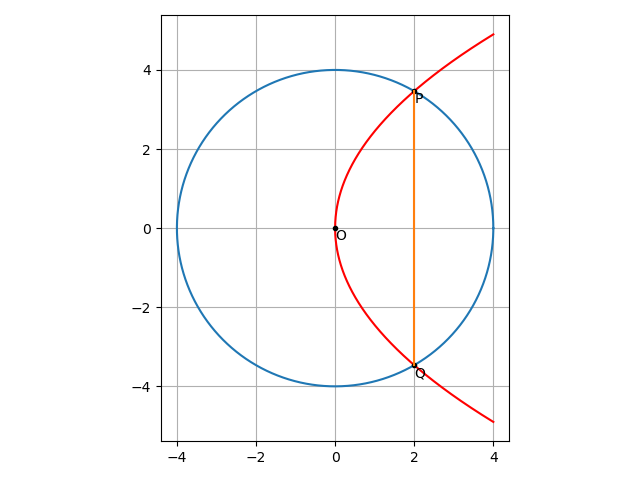
\includegraphics[width=\columnwidth]{figs/parab_circ.png}
        \caption{The conics meet at points $P$ and $Q$.}
        \label{fig:parab-circ}
    \end{figure}
\end{enumerate}
\end{document}
